\chapter{Hardware}\label{Hardware}

\begin{minipage}{12cm}\textit{Se lo si desidera, utilizzare questo spazio per inserire un breve riassunto di ci\`o che verr\`a detto in questo capitolo. Inserire solo i punti salienti.}
\end{minipage}

\vspace*{1cm}


\section{Trasformatore}\label{Trasformatore}

La tesi va scritta usando la terza persona, per quanto possibile, tranne casi veramente eccezionale. In inglese \`e piuttosto standard usare la prima persona (plurale) in testi tecnici. In italiano no.

\section{Driver di Corrente - IBT-2}\label{CurrentDriver}
Per l'attuazione del controllo di corrente nella bobina primaria del trasformatore, è stato usato il driver di corrente \textbf{IBT-2} \cite{IBT-2} .

%todo modificare con Paint.net Per mettere trasformatore e levare linea nera
\begin{figure}[h]
	\centering
	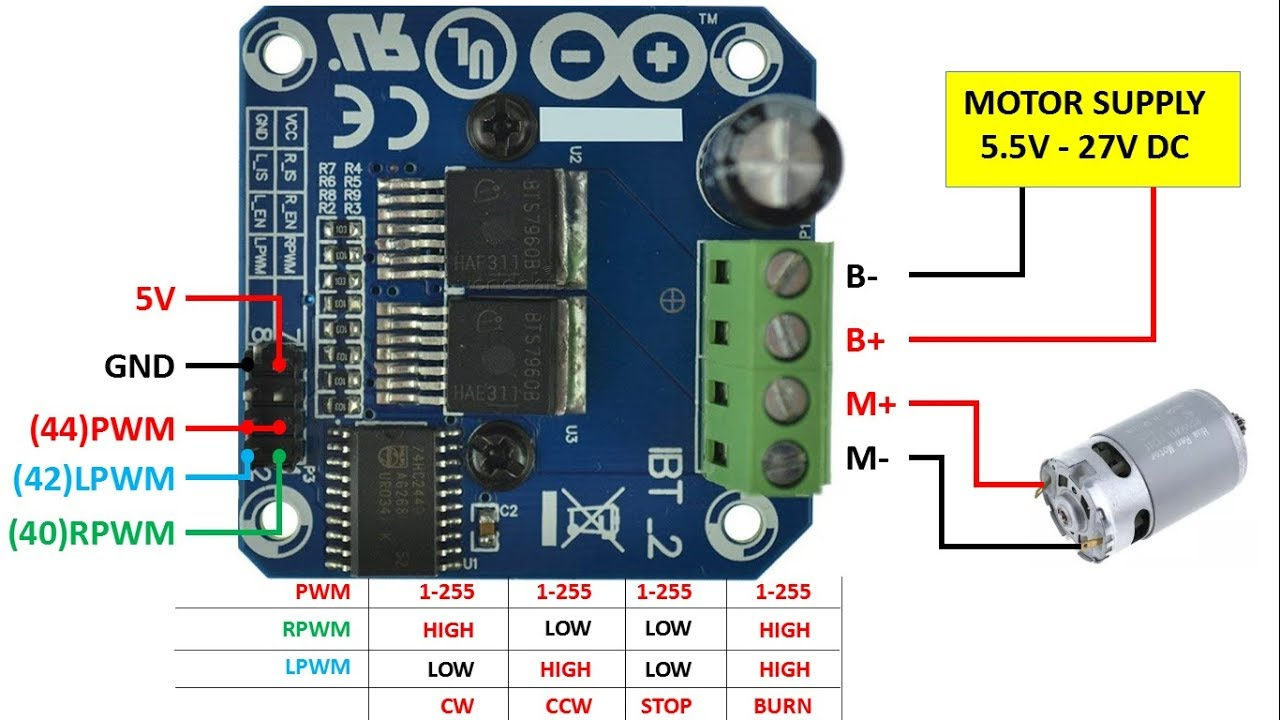
\includegraphics[width=0.6\textwidth]{IBT-2/TopView.jpg}
	\caption[Driver Motori IBT-2 TopView \& PinOut]{IBT-2 TopView.}
\end{figure}

Esso non è un comune Ponte-H, è composto da 2 Half-Bridge collegati insieme mediante una opportuna logica.\\
Questo schema di controllo permette di ottenere prestazioni interessanti dal punto di vista della potenza gestibile:
\begin{enumerate}
	\item Power Input Voltage: 6 ~ 27V
	\item Peak current: 43 A
	\item Massima Frequenza di PWM: 25 kHz
	\item Protezione Sovra Tensioni
	\item Disaccoppiamento Ingresso di Potenza/Logica di controllo
	
\end{enumerate}


\subsection{Non linearità presenti}
asdasdasd

\section{Sensore di Corrente}\label{CurrentSense}

In questa sezione vengono commentate alcune questioni estetiche e di
forma legate alla tesi.


\subsection{Metodo di acquisizione}
asdasd